\documentclass[12pt]{article}
\usepackage{array}
\usepackage{amsmath}
\usepackage{mathtools}
\usepackage{gensymb}
\usepackage{graphicx}
\usepackage{float}
\usepackage{caption}

\allowdisplaybreaks

\begin{document}
    \title{Change in Momentum and Mechanical Energy in Inelastic Collisions}
    \author{Ryan Coyne and Patrick Browning}
    \maketitle
    \section{Abstract}
        The change in momentum and change in mechanical energy was measured for a system of two colliding carts on an air track was. When the mass of the stationary cart was greater than the mass of the moving cart, the changes in momentum and energy were measured to be (-0.0151 \(\pm\) 0.0089) kgm/s and (-0.0100 \(\pm\) 0.0027) J respectively. When the masses were equal the changes in momentum and energy were measured to be (-0.0156 \(\pm\) 0.0015 ) kgm/s and (-0.00990 \(\pm\) 0.00028) J respectively. When the mass of the moving cart was greater than the mass of the stationary cart the changes in momentum and energy were measured to be (-0.017 \(\pm\) 0.049) kgm/s and (-0.0073 \(\pm\) 0.0017) J respectively.
    \section{Introduction}
        In an inelastic collision momentum, given by the equation
        \begin{equation*}
            p = mv
        \end{equation*}
        where m is the mass is conserved which means that the final momentum of the system should be equal to the initial momentum of the system. Therefore the change in momentum should be zero. The system should lose mechanical energy due to the friction between the pin and wax which is what causes the carts to stick together and the collision to be inelastic. The change in mechanical energy is given using the equation
        \begin{equation*}
            \Delta E = \Delta K + \Delta U.
        \end{equation*}
        Where \(\Delta K\) is the change in kinetic energy and \(\Delta U\) is the change in potential energy. Since the interaction is happening on a level track, the change in potential energy will be zero and so \(\Delta E = \Delta K\). This shows that the change in kinetic energy should be negative because the change in mechanical energy should be negative and these quantities are equal.
    \section{Procedure}
        A pin was attached to the end of a cart and wax was attached to the end of a second cart at the same level as the pin on the first cart. A flag was also placed on the top of the first cart for a sonic motion sensor to detect. One hundred grams was added to the second cart and the masses of both carts were determined using a triple beam balance. An air track was leveled by placing the carts on it while it was on and adjusting the height of the legs until the carts would remain in place. The rubber band bumpers were attached to both ends of the track and a sonic motion sensor was placed at one end of the track. 
        
        The carts were place on the track so that the pin of cart one was facing the wax of cart two. Cart one was pulled back against the rubber band bumper while cart two was at rest, approximately 2 thirds of the track length away. The sensor was started and cart one was released. After colliding with cart two the pin stuck into the was so that the carts moved together and impacted the other bumper and then the sensor was stopped. This was done three times while the mass of cart two was greater than cart one. Next, the one hundred grams was removed from cart two and fifty grams was added to cart one and sixty two grams was added to cart two so that the masses would be approximately equal. With these new masses three more trials were conducted in the same way. Finally the extra weight was removed from both carts and one hundred grams was added to cart one and three trials were conducted in the same way again.  
        \begin{figure}[H]
            \centering
            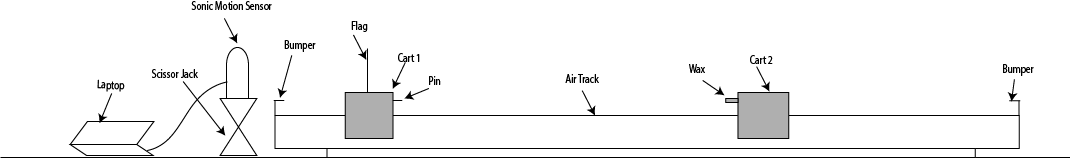
\includegraphics[width=\linewidth]{Setup.png}
            \caption{Experimental Setup}
        \end{figure}
    \section{Data}
        \begin{center}
            \begin{tabular}{ccc|ccc}
                Experiment & \(m_1\) (kg) & \(m_2\) (kg) & Trial & \(v_{i}\) (m/s) & \(v_{f}\) (m/s)\\
                \hline
                \(m_1 < m_2\) & 0.20152 & 0.289155 & 1 & 0.395 & 0.131 \\
                &&& 2 & 0.378 & 0.117\\
                &&& 3 & 0.327 & 0.111\\
                \cline{4-6}
                &&&\(\overline{x}\) & 0.367 & 0.120\\
                &&&\(\sigma_x\) & 0.036 & 0.010\\
                \hline
                \(m_1 = m_2\) & 0.25152 & 0.251155 & 1 & 0.3419 & 0.1436\\
                &&& 2 & 0.3470 & 0.1385\\
                &&& 3 & 0.3440 & 0.1414\\
                \cline{4-6}
                &&&\(\overline{x}\) & 0.3443 & 0.1412\\
                &&&\(\sigma_x\) & 0.0026 & 0.0026\\
                \hline
                \(m_1 > m_2\) & 0.30152 & 0.189155 & 1 & 0.291 & 0.147 \\
                &&& 2 & 0.264 & 0.121\\
                &&& 3 & 0.293 & 0.150\\
                \cline{4-6}
                &&&\(\overline{x}\) & 0.283 & 0.139\\
                &&&\(\sigma_x\) & 0.016 & 0.016\\
                \hline
            \end{tabular}\\[8pt]
            Table 1. Inelastic Collisions.\\
        \end{center}
        \begin{figure*}[h]
            \centering
            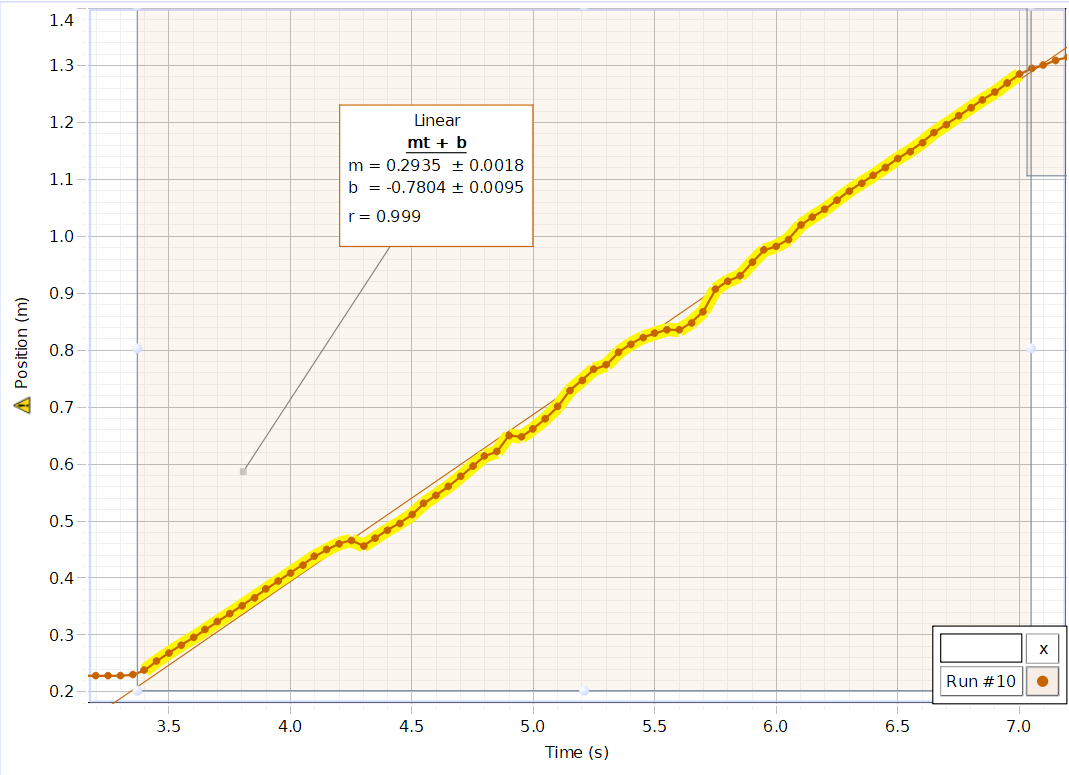
\includegraphics[width=\linewidth]{fit.png}
            \caption{Sample Plot of Position vs Time with Fit to Determine Velocity.}
        \end{figure*}
        \pagebreak
    \section{Calculations}
        \begin{alignat*}{3}
            (1)~
            &&p_i &= m_1v_i\\
            &&p_f &= (m_1 + m_2)v_f\\
            &&\Delta p &= p_f - p_i\\
            &&& = (m_1 + m_2)v_f - m_1v_i\\
            (2)~
            &&\Delta E &= \Delta K + \Delta U\\
            &&K_i &= \frac{1}{2} m_1 v_i^2\\ 
            &&K_f &= \frac{1}{2} (m_1+m_2)v_f^2\\
            &&\Delta K &= \frac{1}{2} (m_1+m_2)v_f^2 - \frac{1}{2} m_1 v_i^2\\
            &&U_i &= 0\\
            &&U_f &= 0\\
            &&\Delta U &= 0\\
            &&\Delta E &= \frac{1}{2} (m_1+m_2)v_f^2 - \frac{1}{2} m_1 v_i^2\\
            (3)~
            &&\sigma^2_{\Delta p} &= \sum_{i=1}^m \left(\sigma_i \frac{\partial \Delta p}{\partial x_i}\right)^2\bigg\rvert_{x=\overline{x}}\\
            &&& = \left(\sigma_{v_i} \frac{\partial \Delta p}{\partial v_i}\right)^2\bigg\rvert_{v_i=\overline{v}_i}+  \left(\sigma_{v_f} \frac{\partial \Delta p}{\partial \overline{v}_f}\right)^2\bigg\rvert_{v_f=\overline{v}_f}\\
            &&\frac{\partial \Delta p}{\partial v_i} &= -m_1\\
            &&\frac{\partial \Delta p}{\partial v_f} &= m_1 + m_2\\
            &&\sigma^2_{\Delta p} &= \left(-\sigma_{v_i}m_1 \right)^2+  \left(\sigma_{v_f} (m_1 + m_2) \right)^2\\
            (4)~
            &&\sigma^2_{\Delta K} &= \sum_{i=1}^m \left(\sigma_i \frac{\partial \Delta K}{\partial x_i}\right)\bigg\rvert_{x=\overline{x}}\\
            &&& = \left(\sigma_{v_i} \frac{\partial \Delta K}{\partial v_i}\right)^2\bigg\rvert_{v_i=\overline{v}_i}+  \left(\sigma_{v_f} \frac{\partial \Delta K}{\partial \overline{v}_f}\right)^2\bigg\rvert_{v_f=\overline{v}_f}\\
            &&\frac{\partial \Delta E}{\partial v_i} &= -m_1v_i\\
            &&\frac{\partial \Delta E}{\partial v_f} &= (m_1+m_2)v_f\\
            &&\sigma^2_{\Delta E} &= (-\sigma_{v_f}\overline{v}_f(m_1+m_2))^2+(\sigma_{v_i}m_1\overline{v}_i)^2\\
            (5)~
            &&\Delta p &= (0.20152~\mathrm{kg}+0.289155~\mathrm{kg})\cdot0.120~\mathrm{m/s}-0.20152~\mathrm{kg} \cdot 0.367~\mathrm{m/s}\\
            &&&= -0.0151\\
            (6)~
            &&-\sigma_{v_i}m_1 &= -0.036~\mathrm{m/s}\cdot 0.20152~\mathrm{kg} \\
            &&& = -0.007255~\mathrm{kgm/s}\\
            && \sigma_{v_f} (m_1 + m_2) &= 0.010~\mathrm{m/s}\cdot (0.20152~\mathrm{kg}+0.289155~\mathrm{kg}\\
            &&& = 0.003093~\mathrm{kgm/s}\\
            &&\sigma_{\Delta p} &= \sqrt{(-0.007255~\mathrm{kgm/s})^2 + (0.003093~\mathrm{kgm/s})^2}\\
            &&&\sqrt{0.0000767~\mathrm{kg^2m^2/s^2}}\\
            &&& = 0.0089~\mathrm{kgm/s}\\
            (7)~
            &&\Delta E &= \frac{1}{2}(0.20152~\mathrm{kg} +0.289152~\mathrm{kg}) \cdot (0.12~\mathrm{m/s})^2-\frac{1}{2}0.20152~\mathrm{kg}(0.367~\mathrm{m/s})^2\\
            &&&=-0.010~\mathrm{J}\\
            (8)~
            && -\sigma_{v_f}\overline{v}_f(m_1+m_2) &= -0.010~\mathrm{m/s} \cdot 0.120~\mathrm{m/s} \cdot (0.20152~\mathrm{kg}+0.289155~\mathrm{kg})\\
            &&&= -0.0005888~\mathrm{J}\\
            &&\sigma_{v_i}m_1\overline{v}_i &= 0.036~\mathrm{m/s}\cdot 0.20152~\mathrm{kg}\cdot 0.367~\mathrm{m/s}\\
            &&&= 0.0026625~\mathrm{J}\\
            &&\sigma_{\Delta E} &= \sqrt{(-0.0005888~\mathrm{J})^2+(0.0026625~\mathrm{J})^2}\\
            &&&=0.0027~\mathrm{J}
        \end{alignat*}
    \section{Conclusion}
        The change in momentum of the system was expected to be zero and it is within three standard deviations of zero when mass one was less than mass two and when mass one was greater than mass two. However, when the masses were equal, the momentum was almost eleven standard deviations away from zero. This is a significant difference. The measurement seems to be in line with the measurements for the other two experiments but the relative error is much smaller. I don't know what could account for this other than random error because the only thing that was changed between the trials were the masses of the carts, for which the relative error is even smaller and would not have an impact on the results. For all three experiments, the change in mechanical energy was several standard deviations less than zero as expected.
\end{document}